\subsection{Explicaci\'on del algoritmo}
La metaheurística de Búsqueda Tabú, se basa en una heurística de Búsqueda Local y permite escapar de los óptimos locales para intentar encontrar mejores soluciones. Incorpora estructuras de memoria para llevar un registro que permite elegir vecindades evitando aquellas que ya fueron visitadas (de esta manera no se forman ciclos). Esta estructura es llamada lista Tabú, debemos definir que información de las soluciones que visitamos va a almacenar y en qué medida.

En nuestro algoritmo para implementar la lista Tabú primero pensamos en guardar las soluciones que iban surgiendo, pero fue descartada porque el número de soluciones que visitamos puede ser muy grande, si pensamos en que las cliques son conjuntos de nodos, entonces se podrían formar muchas combinaciones que tendremos que evaluar al momento de obtener un candidato.
Finalmente nos decantamos por almacenar nodos visitados, que nos permite acotar la lista en el número de nodos del grafo. Un nodo ingresa a la lista Tabú si fue apartado de la solución en el movimiento de una solución a una vecina. 

Por medio de un esquema podemos mostrar el funcionamiento de la metaheurística:
\begin{center}
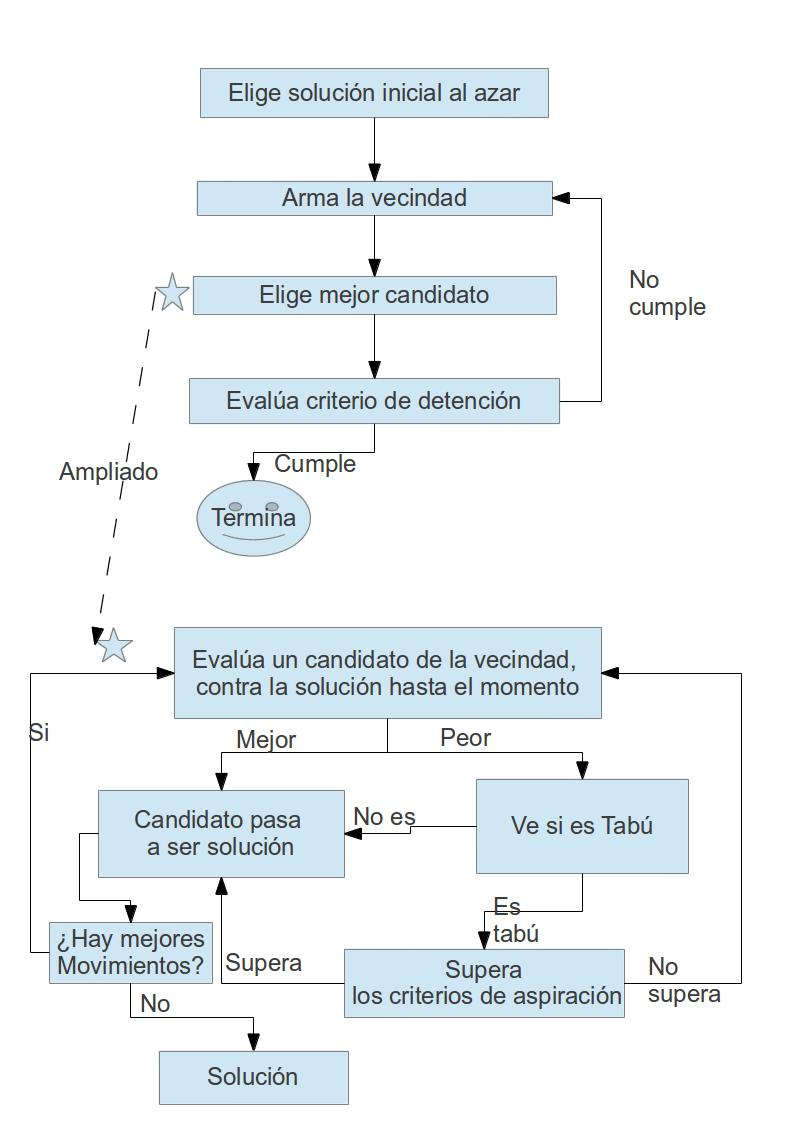
\includegraphics[scale=0.3]{tabu/esquema.jpg}
\end{center}

El criterio de terminación que elegimos, está ligado al número de aristas del grafo. Una vez que encuentra un óptimo local, sigue buscando otras soluciones en una cantidad de iteraciones equivalente a una fracción del total de aristas, esta fracción puede ser modificada en el código si lo precisamos para alguna familia en particular.
Además el criterio de aspiración que empleamos consiste en que si el vecino analizado es mejor que la solución hasta el momento, no importa si forma parte de la lista Tabú o no, se toma como solución. Y cuando todas nuestras posibilidades pertenecen a la lista Tabú, elegimos una de ellas al azar.

\subsection{Pseudoc\'odigo y complejidad}
Este algoritmo utiliza muchas de las funciones de búsqueda local, no agregamos el pseudocódigo de estas para no ser repetitivos, ya que los cambios son mínimos y son respecto a la lista tabú.

\begin{algorithm}
	\caption{Tabú Search}\label{tabu}
	\begin{algorithmic}[1]
	\Procedure{Tabu }{$G\ =\ (V,\ E)$}
		\State $CMF=\ random(nodos)$	\Comment{elige un nodo al azar}
		\State $Clique=\ CMF$
		\State $lista_tabu=\ vacio$
		\While{$nro\_iteraciones\ \leq\ |E|$}
			\State $armar\_vecindad(Clique)$
			\ForAll{$vecino\ in\ vecindad$}
				\If{$frontera(vecino)\ >\ frontera(CMF)$} \Comment{si es mejor que la mejor solución hasta el momento lo cambia sin importar si es tabú}
					\State $CMF=\ vecino$
					\State $Clique=\ CMF$ 
					\State $Actualizar\_lista\_tabu$
				\EndIf
			\EndFor
		\EndWhile

		\If{$CMF\ no\ cambio$}
			\If{$\exists \ vecino\_no\_tabu$}
				\State $Clique=\ vecino\_no\_tabu$
				\State $Actualizar\_lista\_tabu$
			\Else
				\State $Clique=\ algun\_vecino$
			\EndIf
		\EndIf
	\EndProcedure
\end{algorithmic}
\end{algorithm}


\subsection{Casos nefastos}
Los casos en que el tabú search falla son los que para llegar al óptimo debe realizar más cantidad de iteraciones sin modificar el CMF actual que la cota puesta en el while. En el peor caso retorna lo mismo que búsqueda local si arrancan por el mismo nodo. Dado que la solución inicial influye en el hallazgo del óptimo, no podemos asegurar para un caso particular que encuentre el óptimo o no porque nuestra solución inicial es un nodo random.


%\subsection{Experimentaci\'on}




